\chapter{Funktionsweise}\label{ch:operatingPrinciple}

Obwohl Daten im Computer als Bits vorliegen, werden beim Reed-Solomon-Verfahren die zu übermittelnden oder zu speichernden Daten nicht direkt als Bitstrom verarbeitet.
Die zu codierenden Nachrichten werden in Symbole $m_{i}$ der Länge 8 Bit zusammengefasst.
Die Anzahl dieser Symbole ist dann die Nachrichtenlänge $k$ \cite{rileyReedSolomonCodes}.
Eine Nachricht $m$ hat also die Form $[m_{0}m_{1}m_{2}...m_{k-1}]$.

Zum Beispiel wird eine Nachricht mit dem Bitmuster $0010100110100101$ in $00101001\ 10100101$ zerlegt und einzeln in Symbole übersetzt (hier Dezimaldarstellung) $41\ 165$. Hier wäre die Nachrichtenlänge 2.

Nach Hinzufügen der Redundanzsymbole durch Encodieren entsteht ein Block der Länge $n$.
Die Spezifikation der Ausprägung des eingesetzten Reed-Solomon-Codes wird typischerweise als $RS(n, k)$ dargestellt.
Beim Empfänger kommt dann nach dem Decodieren die eventuell Fehler-korrigierte Originalnachricht an \cite{hubertPracticalReedSolomonProgrammers2021}.

\begin{figure}[h]
	\centering
	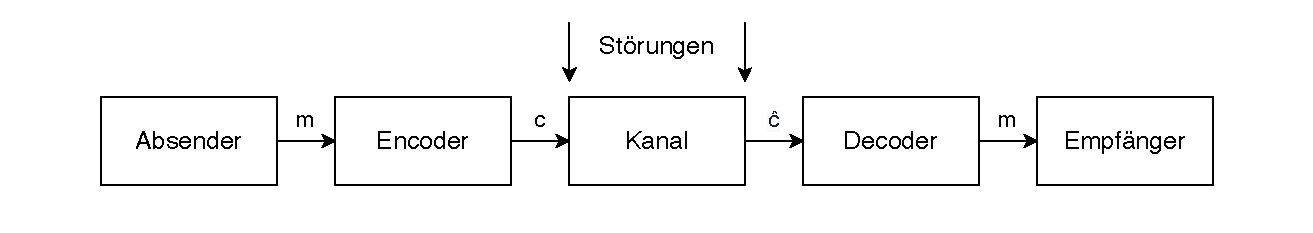
\includegraphics[width=1\textwidth]{figures/Kanalcodierung.drawio.pdf}
	\caption{Ablauf der Kanalcodierung}
	\label{fig:channelcoding}
\end{figure}

Die Berechnungen erfolgen dabei in dem endlichen Körper $GF(2^r)$ über $\mathbb{Z}_2$, dem Lieblingsring im Computer, der genau $2^r=n$ Elemente hat.
Diese Elemente lassen sich als Potenzen einer primitiven Einheitswurzel über einem geeigneten irreduziblen Polynom generieren \cite{weitzKonkreteMathematikNicht2021}.

Diese mathematischen Grundlagen gelten für alle Reed-Solomon Varianten. 
Eine Erklärung des auf dem \acrshort{bch}-Schema basierenden Reed-Solomon-Codes findet sich in Anhang \ref{app:bch-rs}.
Die folgenden Ausführungen zum Encodierung in Abschnitt \ref{sec:encoding} und Decodierung in Abschnitt \ref{sec:decoding} beziehen sich auf den ursprünglichen Ansatz von 1960.

\section{Encodierung}\label{sec:encoding}

Aus einer Nachricht  $m=[m_{0}m_{1}m_{2}...m_{k-1}]$ entsteht das Polynom \[p(x)=\sum_{i=0}^{k-1}m_ix^i=m_0+m_1x+m_2x^2+...+m_{k-1}x^{k-1}\] mit den Nachrichtensymbolen $m_i$ als Koeffizienten der einzelnen Summanden.
Dieses Polynom wird auch als Nachrichtenpolynom bezeichnet \cite{reedPolynomialCodesCertain1960}.
Dieses Nachrichtenpolynom wird bei anderen Reed-Solomon-Varianten auch mit andern Methoden wie zum Beispiel Lagrange-Interpolation generiert \cite{wendlingIntroductionReedSolomon2017}.

Für alle Nachrichten wird ein Codewort $c=[c_{0}c_{1}c_{2}...c_{n-1}]$ der Länge $n=k+2t$ generiert, wobei $k$ die Länge der ursprünglichen Nachricht und $2t$ die Anzahl der redundanten Symbole ist \cite{verbeureReedSolomonErrorCorrecting2022}. 
Dadurch können $2t$ Fehler erkannt und $t=\lfloor\frac{n-k}{2}\rfloor$ Fehler korrigiert werden (Beweis siehe Anhang \ref{app:hammingDistanceRS}).
Das Codewort entsteht durch das Einsetzten von $n$ festen Werten in das Nachrichtenpolynom.
\[
\makebox[\linewidth]{%
	\hfill
	$c_0=p(0);\,c_i=p(\alpha^i)$\hfill
	\llap{($i\in\{1;\dots;n-2\}$)}%
}
\]
Diese Werte $[0\,\alpha^0 \alpha^1 \alpha^2...\alpha^{n-2}]$ sind die Potenzen einer primitiven Einheitswurzel des endlichen Körpers $GF(2^r)=GF(n)$ zuzüglich der 0, also alle Elemente des Körpers \cite{weitzKonkreteMathematikNicht2021}.
Dieses Codewort wird dann gespeichert oder übertragen.
Im Kanal können vor dem Decodieren Störungen das Codewort verfälschen.

\section{Decodierung}\label{sec:decoding}

Aus dem Codewort $c=[c_{0}c_{1}c_{2}...c_{n-1}]$ wird durch Decodieren die ursprüngliche Nachricht wiederhergestellt.
Dazu muss die Encodierung rückgängig gemacht werden, indem für jedes Symbol die Encodierungsgleichung aufgestellt wird. 
Allerdings ist nun $p(x)$ unbekannt und soll mit Hilfe der $\alpha^i$ und der empfangenen $c_i$ durch $c_0=p(0)$ und $c_i=p(\alpha^{i-1})$ berechnet werden \cite{reedPolynomialCodesCertain1960}.
Dadurch entsteht ein Gleichungssystem mit $n$ Gleichungen und $k$ Unbekannten.
\begin{alignat}{5}
	&c_0&&=p(0)&&=m_0\nonumber\\
	&c_1&&=p(\alpha^0)&&=m_0+m_1&&+m_2&&+\cdots+m_{k-1}\nonumber\\
	&c_2&&=p(\alpha^1)&&=m_0+m_1 \alpha&&+m_2 (\alpha)^2&&+\cdots+m_{k-1} (\alpha)^{k-1}\nonumber\\
	&c_3&&=p(\alpha^2)&&=m_0+m_1 \alpha^2&&+m_2 (\alpha^2)^2&&+\cdots+m_{k-1} (\alpha^2)^{k-1}\nonumber\\
	&&&&&&&\cdots\nonumber\\
	&c_{n-1}&&=p(\alpha^{n-2})&&=m_0+m_1 \alpha^{n-2}&&+m_2 (\alpha^{n-2})^2&&+\cdots+m_{k-1} (\alpha^{n-2})^{k-1}\nonumber
\end{alignat}
Die unbekannten Koeffizienten des Polynoms sind gesuchten Nachrichtensymbole $m_i$. 
Da $n>k$, reichen $k$ dieser Gleichungen aus, um das Gleichungssystem eindeutig zu lösen und so die Nachricht zu erhalten.

Allerdings ist das Codewort möglicherweise fehlerbehaftet. 
Einige Symbole von $c$ können also verändert worden sein, sodass ein $\hat{c}$ entsteht und die dazugehörige Gleichung falsch ist \cite{verbeureReedSolomonErrorCorrecting2022}.
Werden eine oder mehrere falsche Gleichungen in einem Gleichungssystem verwendet, liefert dieses veränderte Koeffizienten und somit eine falsche Lösung $\hat{m}$.

Wie viele Fehler und an welchen Stellen diese aufgetreten sind lässt sich nicht a priori nicht sagen. 
So reicht es also nicht aus, nur $k$ Gleichungen zum Lösen des Gleichungssystems zu verwenden, da in diesen $k$ Gleichungen bis zu $2t$ Fehler enthalten sein können.
Um eine korrekte Lösung des Gleichungssystems zu finden, müssen alle $\binom{n}{k}$ möglichen Gleichungssysteme gelöst werden.
So ergeben sich mindestens $\binom{n-t}{k}$ Gleichungssysteme mit identischer Lösung, da diese die richtige ist \cite{reedPolynomialCodesCertain1960}.
Die Lösung der restlichen, fehlerbehafteten Gleichungssysteme variiert und gleiche Ergebnisse treten selten auf.
Es wird gezählt, wie viele Gleichungssysteme eine bestimmte Lösung liefern und so wird das Ergebnis, welches am häufigsten aufgetreten ist, ausgewählt. 
So kann die Nachricht $m$ aus dieser Lösung, den $m_i$, wiederhergestellt werden.
Bei dem Verfahren wird vorausgesetzt, dass nie mehr als $2t$ Fehler auftreten, da sonst das eben beschriebene Lösungs-Auswahlverfahren fehlschlagen würde.
Eine beispielhafte Durchführung dieses Verfahrens findet sich in Anhang \ref{app:example}.

Es gibt kein Verfahren, das mehr Fehler korrigieren kann als der Reed-Solomon-Code.
Das beweist der Hamming-Abstand, eine Kenngröße für die Effektivität von Codierungsverfahren, der bei Reed-Solomon $n-k+1$ ist \cite{reedPolynomialCodesCertain1960}.
Unter dem Hamming-Abstand eines Codes versteht man das Minimum aller Abstände zwischen verschiedenen Wörtern innerhalb des Codes.
Bei Codes mit Hamming-Abstand $h$ können alle $(h-1)$-Bit-Fehler erkannt werden, also bei Reed-Solomon $n-k=2t$.
Ein ausführlicher Beweis dazu findet sich in Anhang \ref{app:hammingDistanceRS}.
Das Verfahren schafft demnach den optimalen Kompromiss zwischen der Länge der hinzugefügten Redundanz und der Fähigkeit, Fehler zu erkennen und zu korrigieren.
Die Singleton-Schranke ist die Obergrenze für den Hamming-Abstand und beträgt $n-k+1$ \cite{friedrichsKanalcodierung1996}.
Also kann kein Verfahren effektiver agieren als die Reed-Solomon-Codes.

Im Anhang \ref{app:comparison} findet sich eine Vergleichstabelle, in der der Reed-Solomon-Code mit dem Hamming-Code und dem \acrshort{bch}-Code hinsichtlich ihrer Effektivität anhand von Zahlen verglichen wird.
Der Hamming-Code ist zwar ineffektiver, aber benutzerfreundlicher bei Einzelbitfehlern \cite{williamsHammingCodeFehlererkennungUnd2024}.
Der \acrshort{bch}-Code wird, obwohl er im Verhältnis von Redundanz zu Fehlern nicht so effektvoll ist, bei einigen Anwendungen eingesetzt, da er kostengünstiger zu implementieren ist \cite{schulz-hankeBCHCodesCombined2023}. 

In den 1960ern war dieses effektive Verfahren leider noch nicht effizient einsetzbar, da das Lösen der Gleichungssysteme für größere Werte für $n$ und $k$ lange dauert \cite{verbeureReedSolomonErrorCorrecting2022}. 
Wenn man beispielsweise eine typische Konfiguration $RS(255,223)$ aus dem Voyager-Programm annimmt, folgen daraus $\binom{255}{223}\approx5\cdot 10^{40}$ Gleichungssysteme, die gelöst werden müssen.
Bei einer Lösungsdauer von einer Millisekunde pro Gleichungssystem, wären das immer noch eine Gesamtdauer von ca. $3,17\cdot10^{29}$ Jahren. 
So kann man leicht nachvollziehen warum dieses Verfahren in dieser Form nicht effizient lösbar ist.

\section{Berlekamp-Welch Algorithmus}\label{sec:bwAlgo}

Der Berlekamp-Welch Algorithmus bietet eine Lösung dieses Problems. 
Dazu wird ein Fehlerlokalisierungspolynom $e(x)=(x-e_1)(x-e_2)\cdots(x-e_t)$ mit $deg(e)=t$ definiert, wobei die $e_i$ die Stellen sind, an denen Fehler aufgetreten sind \cite{weitzKonkreteMathematikNicht2021}.
So is $e(x)$ an dem Fehlerstellen gleich 0.
Außerdem wird $q(x)=p(x)e(x)$ mit $deg(q)=deg(p)+deg(e)=k-1+t$ gebildet.
Umgeformt sind die zu bestimmenden Polynome
\begin{alignat}{1}
	&e(x)=1x^t+b_{t-1}x^{t-1}+\cdots+b_1x+b_0\nonumber\\
	&q(x)=a_{k+t-1}x^{k+t-1}+a_{k+t-2}x^{k+t-2}+\cdots+a_1x+a_0,\nonumber
\end{alignat}
welche zusammen $k+2t$ unbekannte Koeffizienten haben.
Die $k+2t$ Symbole des Codeworts liefern also genau genug Informationen um diese Koeffizienten eindeutig zu bestimmen, indem man $k+2t$ Gleichungen der Form $q(i)=e(i)$ aufstellt, wobei $1\leq i\leq k+2t$.
Mit diesen gegebenen Koeffizient sind auch $q(x)$ und $e(x)$ bekannt und es kann durch Polynomdivision wieder das ursprüngliche Polynom $p(x)$ berechnet werden, um damit die Nachricht wie bei der Encodierung zu bestimmen \cite{fengBerlekampWelchAlgorithmGuide}.

\section{Hardware-Implementierung}\label{sec:hardware}

Um dieses Fehlerkorrekturverfahren in möglichst vielen Szenarien anwenden zu können, ist es wichtig, dass die Verwendung fast ohne Beeinträchtigung möglich ist.
Dafür wird häufig auf eine spezielle Implementierung in Hardware gesetzt, um den Einsatz auch auf kleinen Geräten wie Mikrokontrollern zu ermöglichen.
Da viele Reed-Solomon-Codes auf der Polynomdivision basieren, gibt es dafür dedizierte Hardwarekomponenten \cite{verbeureReedSolomonErrorCorrecting2022}.
Eine solche Implementierung zur Polynomdivision, wie in Abbildung \ref{fig:polynomdivCircuit} abgebildet, wird im Folgenden näher beschrieben.
\begin{figure}[ht]
	\centering
	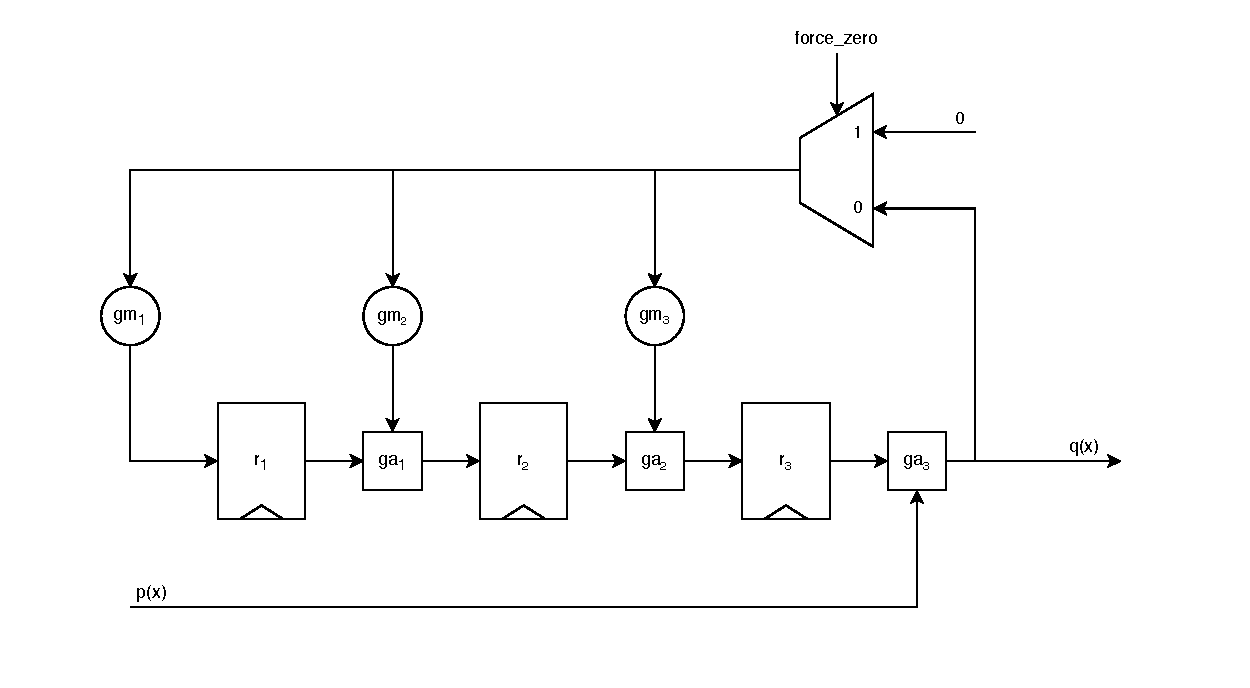
\includegraphics[width=0.9\textwidth]{figures/Polynomdivision-Hardware.drawio.pdf}
	\caption{Schaltung zur Polynomdivision}
	\label{fig:polynomdivCircuit}
\end{figure}
Die Schaltung arbeitet mit Galois-Addierern $ga_i$ und Galois-Multiplizierern $gm_i$ und ist rückgekoppelt, das heißt die Berechnungen basieren auf dem zuvor durchgeführten Berechnungsschritt \cite{masseyShiftregisterSynthesisBCH1969}.
Am Eingang $p(x)$ werden jeweils die Koeffizienten des Dividenden angelegt, am Ausgang $q(x)$ kommen die Koeffizienten des Ergebnisses an, jeweils die Koeffizienten mit dem höchsten Exponenten zu erst.
Der Divisor ist durch die Multiplizierer dargestellt.
Die $gm_i$ enthalten jeweils den $i$ten Koeffizienten des Divisors und multiplizieren diesen mit ihrem Eingang.
Bei $gm_0$ handelt es sich um den Koeffizienten von $x^0$. 
Die Addierer addieren ihre jeweiligen Eingänge und geben sie an ihrem Ausgang aus.
Dabei werden die Reste eines Divisionsschrittes in den Registern $r_i$ gespeichert und sequenziell in den folgenden Iterationen weiterverwendet, so wie man die Polynomdivision auch mit Stift und Papier durchführen würde.
Die Schaltung in der Abbildung ist der Übersichtlichkeit halber nur für einen Divisor mit drei Summanden dargestellt.
In der Realität müssten, für das konkrete Verfahren angepasst, entsprechend mehr Komponenten verbaut sein.

Durch das Verwenden von Galois-Multiplizierern und -Addierern entsteht ein Vorteil gegen über der klassischen Arithmetik, denn die Ergebnisse bleiben innerhalb dieses Körpers und benötigen also immer die gleiche Anzahl an Speicherplatz \cite{weitzKonkreteMathematikNicht2021}.
Dadurch können die Komponenten wie Register und verbindende Busleitungen auf eine konkrete Bit-Anzahl angepasst werden, womit keine kostspielige Hardware verbaut sein muss und diese dann optimal ausgenutzt wird.
Außerdem können diese Schaltungen mit einfachen logischen Gatter umgesetzt werden \cite{biernatHardwareImplementationReedSolomon2010, southwellIntroductionErrorDetection}.
Ein Galois-Addierer wird zum Beispiel durch ein XOR-Gatter implementiert.

Mit Hilfe dieser oder ähnlicher Schaltungen und dem in Abschnitt \ref{sec:bwAlgo} genannten Algorithmus war es möglich, Reed-Solomon in den verschiedensten Einsatzbereichen zu verwenden, wie im nächsten Kapitel erläutert wird.